\section{Constructing Ladder Operator Block-Encodings}
\label{sec:ladder-op-oracles}

In this work, we are focused on generating block-encodings for second-quantized Hamiltonians that include both fermions and bosons.
In the previous section, we discussed a block-encoding framework for constructing a block-encoding of an operator described as a linear combination of operators assuming one has access to block-encodings of the operators comprising the linear combination.
In this section, we discuss the construction of these block-encodings for ladder operators, products of ladder operators, and particular linear combinations of ladder operators acting on fermionic and bosonic modes.

First, we discuss the encoding that we choose to represent the fermionic and bosonic modes since different system encodings will require different block-encodings constructions.
Then we will present schemes for constructing controlled block-encodings of both fermionic and bosonic ladder operators.
We include control qubits in our constructions since these block-encodigns will often be applied under some coherent control structure and controlling operations can sometimes singificantly increase the cost of the operation.
Finally, we discuss how these block-encodings can be efficiently combined to give block-encodings of a product of ladder operators or a ``term'' as defined by Eq. \ref{eq:term} and particular linear combinations of ladder operators.   

\subsection{Encoding}
\label{subsec:encoding}

In this work, the encoding that is used for the occupation of the fermionic modes is identical to the Jordan-Wigner encoding \cite{jordan-wigner}.
The map between a Fock state to a qubit state is given as 
\begin{equation}
    \ket{n_{I_b}, \dots, n_{1_b}, n_{0_b}} \rightarrow \ket{q_{I_b}, \dots, q_{1_b}, q_{0_b}}
\end{equation}
where $n_{i_b} = q_{i_b} \in [0, 1]$ depending on if mode $i$ is occupied or not.
The encoding scheme is the same for antifermions.
In total, the number of qubits required for the fermionic and antifermionic susbsystems is: $Q_{\psi_b} = I_b$ and $Q_{\psi_d} = I_d$.

The encoding scheme for bosons must allow for occupancies in the range $[0, \Omega]$ due to the absence of the Pauli exclusion principle.
We choose to represent store the occupancy of a bosonic mode in binary notation: 
\begin{equation}
    \ket{n_{i_a}} \rightarrow \ket{b_j, b_{j-1}, ..., b_0}
\end{equation}
where $j$ runs from $0$ to $\lceil \log_2{\Omega} \rceil - 1$ and the values of $b_j$ are given by the binary representation of $n_{i_a}$.
This is identical to the encoding used in \cite{rhodes2024exponential}. \ws{check citation}

Storing the occupation of each bosonic mode requires $\lceil \log_2{\Omega} \rceil$ qubits if we assume that the maximum bosonic occupation is the same for each bosonic mode.
This choice of the maximum bosonic occupation being constant for all bosonic modes is not a restriction of the methods presented in this work, but is chosen for simplicity. 
With this choice, the number of qubits required for the bosonic subsystem is: $Q_{\psi_a} = I_a \lceil \log_2{\Omega} \rceil$.

\subsection{Fermionic Ladder Operators}
\label{subsec:fermionic-be}

In this section, we aim to define a family of unitaries ($\{U_{b^\dagger_i}, U_{b_i}\}$) that generate block-encodings of the associated fermionic creation ($b_i^\dagger$) and annihilation ($b_i$) operators.
As these are block-encodings of non-unitary operators, we define the associated unitary operators to be of the form of Eq. \ref{eq:general-block-encoding}:
\begin{equation}
    U_{b^\dagger_i} \ket{\psi} \ket{0}_\text{anc} = b^\dagger_i \ket{\psi}\ket{0}_\text{anc} + \beta_\psi \ket{\text{junk}}\ket{0_\perp}_\text{anc}
\end{equation}
Since the fermionic ladder operators are already scaled such that their spectral norm is less than $1$, we do not need to introduce any rescaling factor for these operators.

The definition of the fermionic creation operator (Eq. \ref{eq:fermionic-creation}) creates two implications.
First, if the mode is already occupied, then state in our encoded subspace should be zeroed-out. 
Second, if the mode is unoccupied, then the mode should become occupied and a sign should be applied based on the occupancy of the preceeding fermionic modes.
Therefore, the action of our unitary will need to be controlled based on the occupation of the fermionic mode:
\begin{equation}
    U_{b^\dagger_i} \ket{\psi_i} \ket{0}_\text{anc} =
    \begin{cases} 
        (-1)^{\sum_{j < i} n_{b_j}} \ket{1} \ket{0}_\text{anc} & \text{when $\ket{\psi_i}$ is $\ket{0}$} \\
        \ket{\text{junk}} \ket{1}_\text{anc} & \text{when $\ket{\psi_i}$ is $\ket{1}$} \\
    \end{cases}
\end{equation}

\begin{figure}[h]
    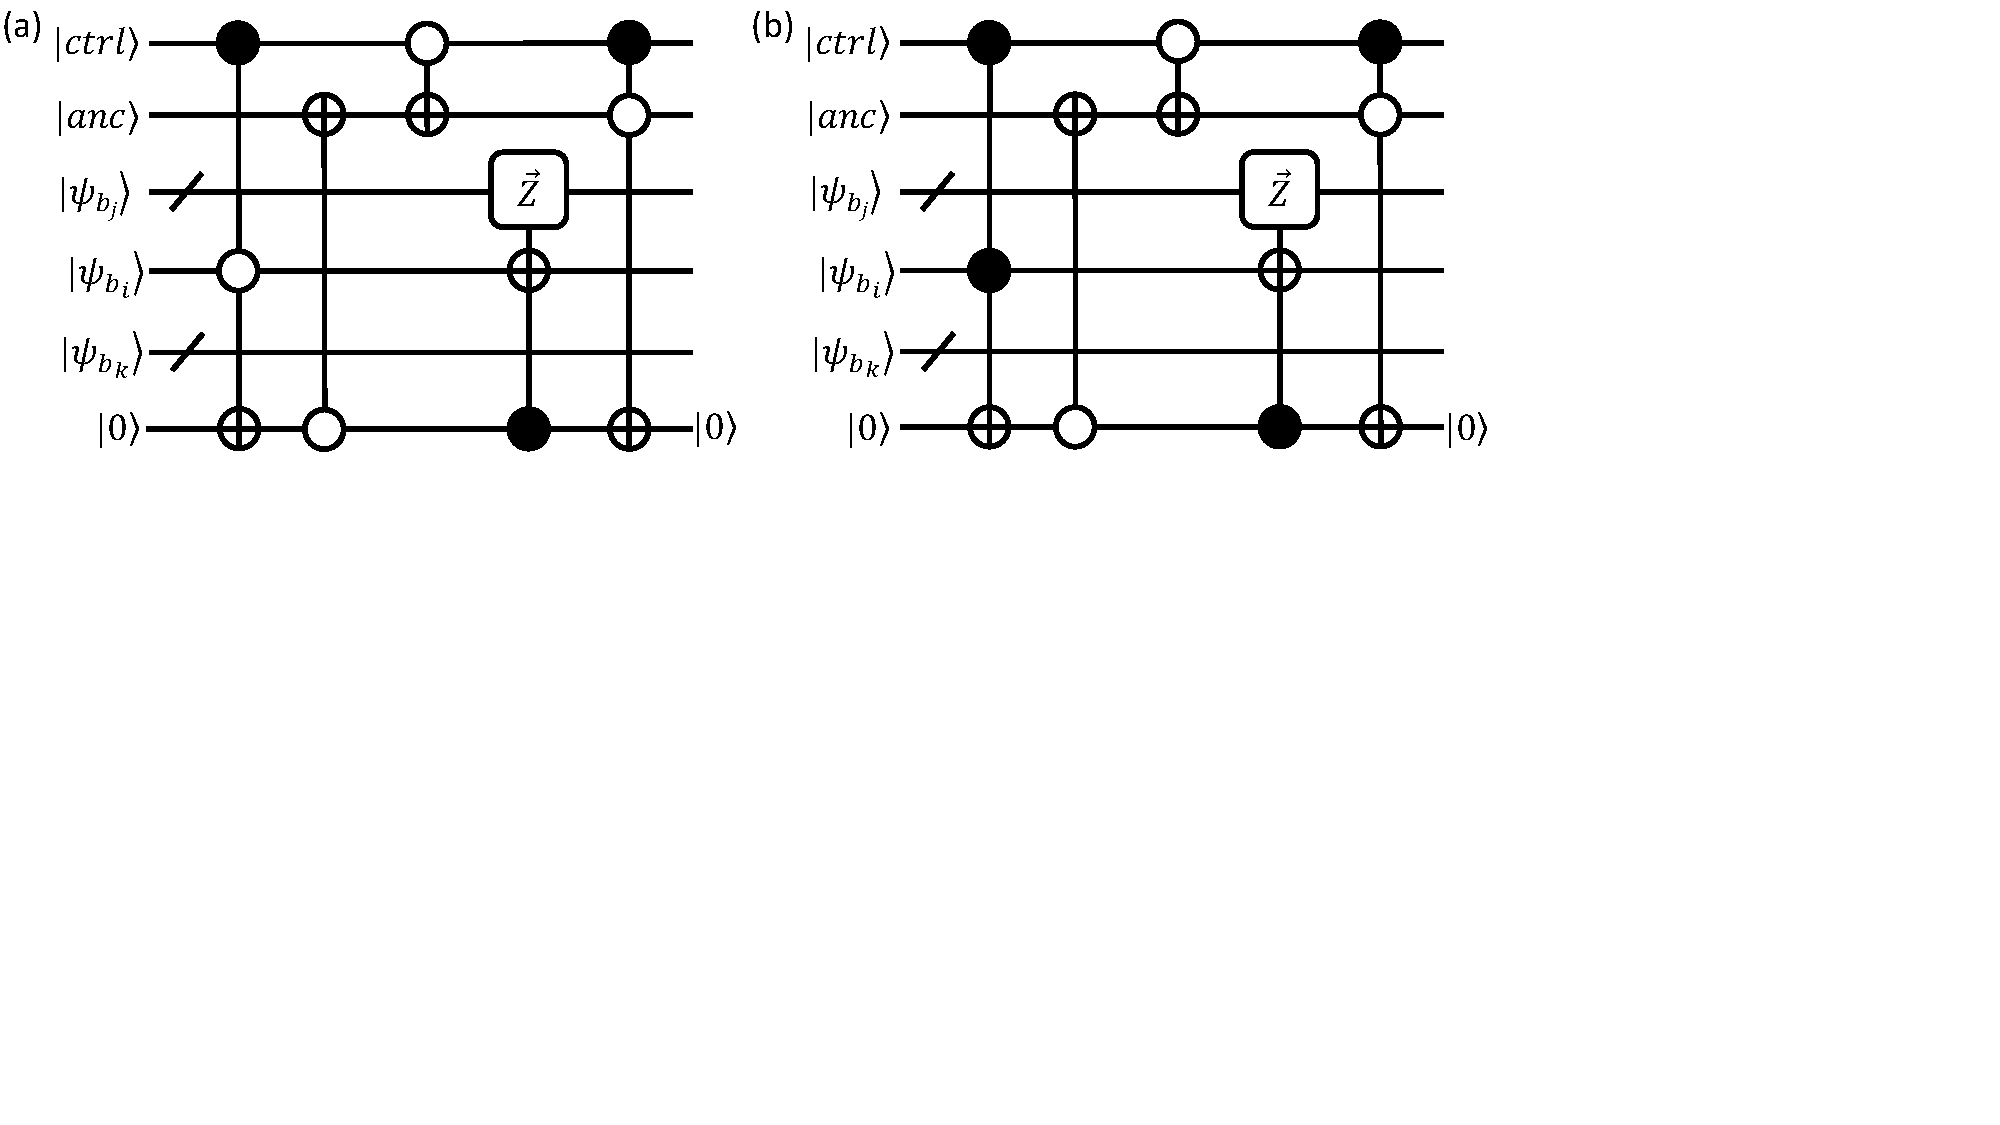
\includegraphics[width=12cm]{figures/fermionic-be.pdf}
    \caption{
        \textbf{Block-Encoding Fermionic Ladder Operators}
        In subfigure a, a block-encoding for the fermionic creation operator acting on the $i^\text{th}$ mode is given.
        In subfigure b, a block-encoding for the fermionic annihilation operator acting on the $i^\text{th}$ mode is given.
        The clean ancilla (low qubit) is initialized using a left-elbow and stores the $\ket{1}$ state if and only if the control is on (operator should be applied) and the occupation of the $i^\text{th}$ mode indicates that the operator will not zero-out the state.
        For a creation (annihilation) operator, the state will not be zeroed-out if the mode is unoccupied (occupied).
        If the clean ancilla is off, the block-encoding ancilla ($\ket{\text{anc}}$) is flipped outside of the encoded subspace $\ket{1}$.
        If the control is off, the block-encoding ancilla is flipped again so that it remains in its original state.
        The state is then updated accordingly if the clean ancilla is in the $\ket{1}$ state.
        The state is updated by applying Pauli Z gates to the preceeding fermionic modes to apply the appropriate sign and then applying a Pauli X gate to flip the occupation of the $i^\text{th}$ mode.
        Finally, the clean ancilla is uncomputed such that it is reset to $\ket{0}$.
    }
    \label{fig:fermionic-be}
\end{figure}


In Figure \ref{fig:fermionic-be}a, we show a unitary that implements $U_{b^\dagger_i}$.
The initial Toffoli gate computes the logicial-AND of both the control qubit and the fermionic mode being unoccupied ($\ket{0}$) and stores the value in a clean ancilla qubit.
If these conditions are not both true, then the block-encoding ancilla is flipped to $\ket{1}$ so that the state is outside of the encoded subspace.
Otherwise the block-encoding ancilla is left in the $\ket{0}$ state.
If the control qubit is off, the block-encoding ancilla is flipped again so that it is left in the $\ket{0}$ state regardless of the state of the control qubit.
The sign of the output state can be achieved by applying controlled Pauli-Z operators to each of the fermionic modes with index $j < i$: $\vec{Z}_j$.
The occupation of the fermionic mode is updated using a controlled Pauli-X operator: $X_i$.
Lastly, the ancilla qubit storing the logical-AND is reset to the $\ket{0}$ state using a Toffoli gate.
\ws{The non-Clifford operations for block-encoding of an individual fermionic ladder operator using this construction is 2 Toffoli gates.}

A block-encoding for the fermionic annihilation operator, $U_{b_i}$, can be constructed similarly to $U_{b^\dagger_i}$.
The fermionic creation operator only acts nontrivially when the mode is \textit{unoccupied}.
Inversely, the fermionic annihilation operator will only act nontrivially if the mode is \textit{occupied}.
A circuit implementing $U_{b_i}$ is shown in Figure \ref{fig:fermionic-be}b where the only difference compared to $U_{b^\dagger_i}$ is that the control on the fermionic mode is $1$-controlled instead of $0$-controlled.

 

\subsection{Products of Fermionic Ladder Operators}

In the previous subsection, we gave quantum circuit constructions that block-encode individual fermionic ladder operators.
As noted in subsection \ref{subsec:be-products}, we discussed how we can naively generate a block-encoding for a product of operators using a product of the unitaries that block-encode each operator.
In this subsection, we will give quantum circuit constructions that block-encode products of fermionic ladder operators using fewer quantum resources than are required by this naive strategy.

Each of the block-encoding circuits for individual fermionic ladder operators requires 2 Toffoli gates and one block-encoding ancilla.
If there are $B$ fermionic ladder operatos within a term, then the naive construction will require $2B$ Toffoli gates and $B$ block-encoding ancillae \ws{Gilyén et. al say this should still be $1$ ancilla, but I don't think this is correct.}. 

\begin{figure}[h]
    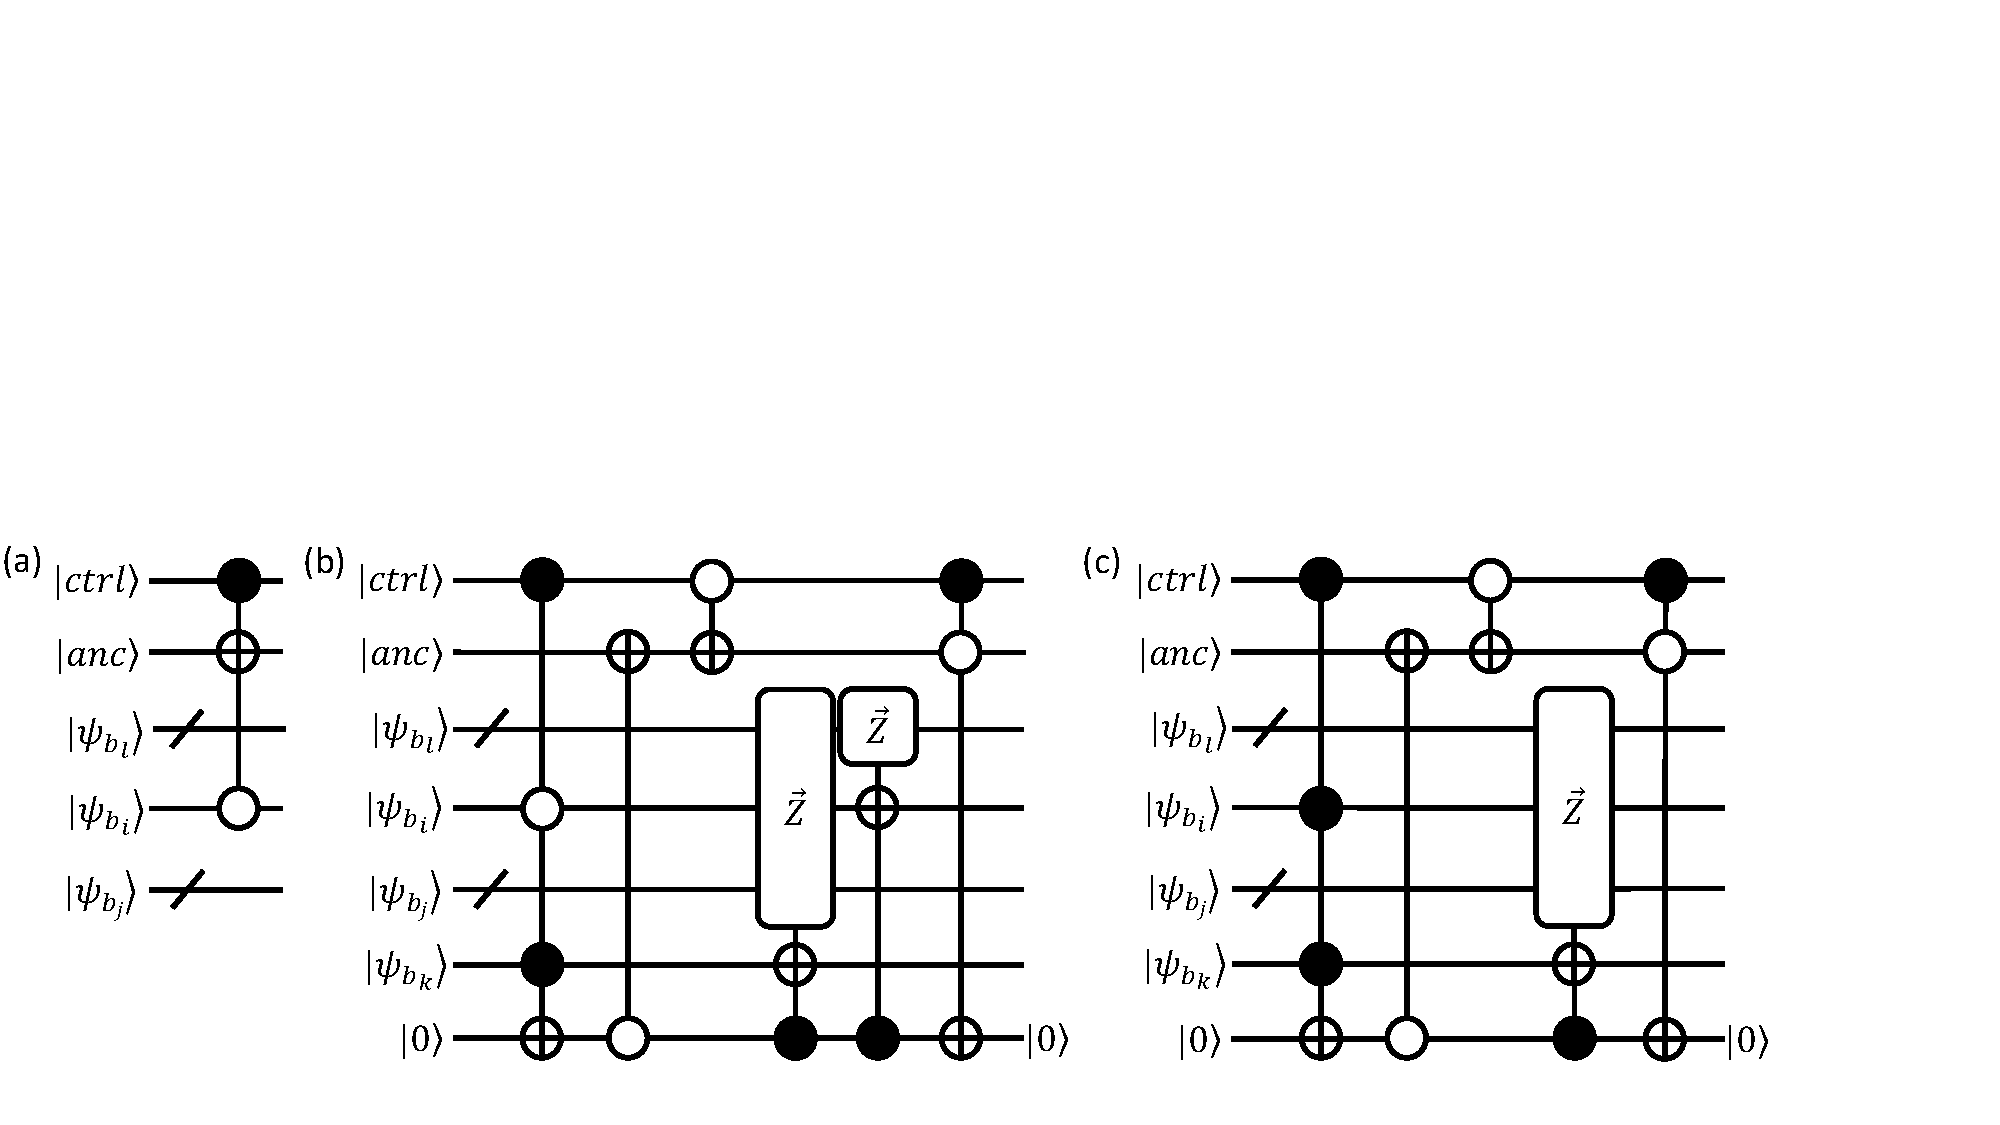
\includegraphics[width=12cm]{figures/fermionic-products-be.pdf}
    \caption{
        \textbf{Block-Encoding Products of Fermionic Ladder Operators}
        In subfigure a, a block-encoding for the fermionic number operator acting on the $i^\text{th}$ mode is given.
        This circuit can be constructed using a single Toffoli gate.
        If the control qubit is active and the $i^\text{th}$ fermionic mode is unoccupied, the ancilla qubit is flipped to push it outside of the encoded subspace.
        In subfigure b, a block-encoding for the operator $b_i^\dagger b_k$ with $i \neq k$ is given.
        In subfigure c, a block-encoding for the operator $b_i^\dagger b_i b_k$ with $i \neq k$ is given.
    }
    \label{fig:fermionic-products-be}
\end{figure}

As a simple example where we can produce a more efficient construction, consider the fermionic number operator: $b_i^\dagger b_i$.
Using the naive construction to block-encode this operator as the product of the block-encodings for $b_i^\dagger$ and $b_i$ separately would require $4$ Toffoli gates and $2$ block-encoding ancillae.
However, if we note the behavior of the conjoined operator on an arbitrary quantum state, we can produce a more efficient block-encoding.
When this operator is applied, the state will be zeroed-out if the $i^\text{th}$ mode is unoccupied.
Alternatively, if the $i^\text{th}$ mode is occupied, then the state is left unchanged.
Therefore, we can block-encode this operator using one Toffoli gate and one block-encoding ancilla as shown in Figure \ref{fig:fermionic-products-be}a.
The Toffoli gate flips the block-encoding ancilla outside the subspace if the $i^\text{th}$ mode is unoccupied to indicate that the state was zeroed-out, but otherwise leaves the state and the block-encoding ancilla unchanged.

For a more general product of two fermionic ladder operators, a block-encoding circuit for the operator $b_i^\dagger b_k$ where $i \neq k$ is given in subfigure \ref{fig:fermionic-products-be}b.
This circuit contains the same structure as the block-encoding circuits for the individual fermionic ladder operators except it includes logic on the occupation of both the $i^\text{th}$ and $k^\text{th}$ modes.
From the operator $b_i^\dagger$ we know that the state will be zeroed-out unless the $i^\text{th}$ mode is unoccupied.
Likewise the operator $b_k$ indicates that the state will be zeroed-out unless the $k^\text{th}$ mode is occupied.
These conditions and the condition on the control qubit can all be included in the initialization of the clean ancilla.
The update of the block-encoding ancilla, the updates on the system registers, and the reset of the clean ancilla can proceed following the same pattern as used for the individual fermionic ladder operator.
% A multi-controlled Toffoli gate with $N$ conditions can be be decomposed into $N-1$ Toffoli gates each with two controls using temporary clean ancillae.
% This decomposition is discussed in more detail in Appendix \ref{sec:elbows}.
This block-encoding circuit requires three Toffoli gates and one block-encoding ancilla.
This construction can be generalized to arbitrary product of $B^*$ ladder operators when each individual ladder operator acts on a different mode.
Each ladder operator will contribute a new control condition on the initialization of the clean ancilla.
Therefore each of these circuits will require $B^* + 1$ Toffoli gates and one block-encoding ancilla.

When multiple ladder operators act on an single mode, we can reduce the cost slightly.
If we assume that the term is normal ordered \ws{@Gus is this assumption necessary for the following statement?}, then the only non-trivial operators that can act on the same mode is an annihilation operator followed by a creation operator: $b_i^\dagger b_i$.
As noted, this is a number operator on the $i^\text{th}$ mode and we described its action above where it will zero-out the state if the fermionic mode is unoccupied and otherwise leaves the state unchanged.

A block-encoding of an operator of the form $b_i^\dagger b_i b_k$ can be achieved using the circuit shown in subfigure \ref{fig:fermionic-products-be}c.
This circuit is constructed using similar logic regarding which occupation states of the $i^\text{th}$ and $k^\text{th}$ modes result in the state not being zeroed-out.
For the $i^\text{th}$ mode, the state is not zeroed-out if the mode is occupied and no update on the $i^\text{th}$ fermionic mode is required. 
The updates of the block-encoding ancilla, the update of the system for $b_k$, and the reset of the clean ancilla can be performed in the same way as the previous block-encoding circuits.
The non-Clifford cost of these circuits is dependent on the number of fermionic modes that are active (have a ladder operator acting on them) within the term as opposed to the total number of operators.
If $B$ is the number of active fermionic modes in the term, then these block-encoding circuits require $B + 1$ Toffoli gates and one block-encoding ancilla. 


\begin{figure}[h]
    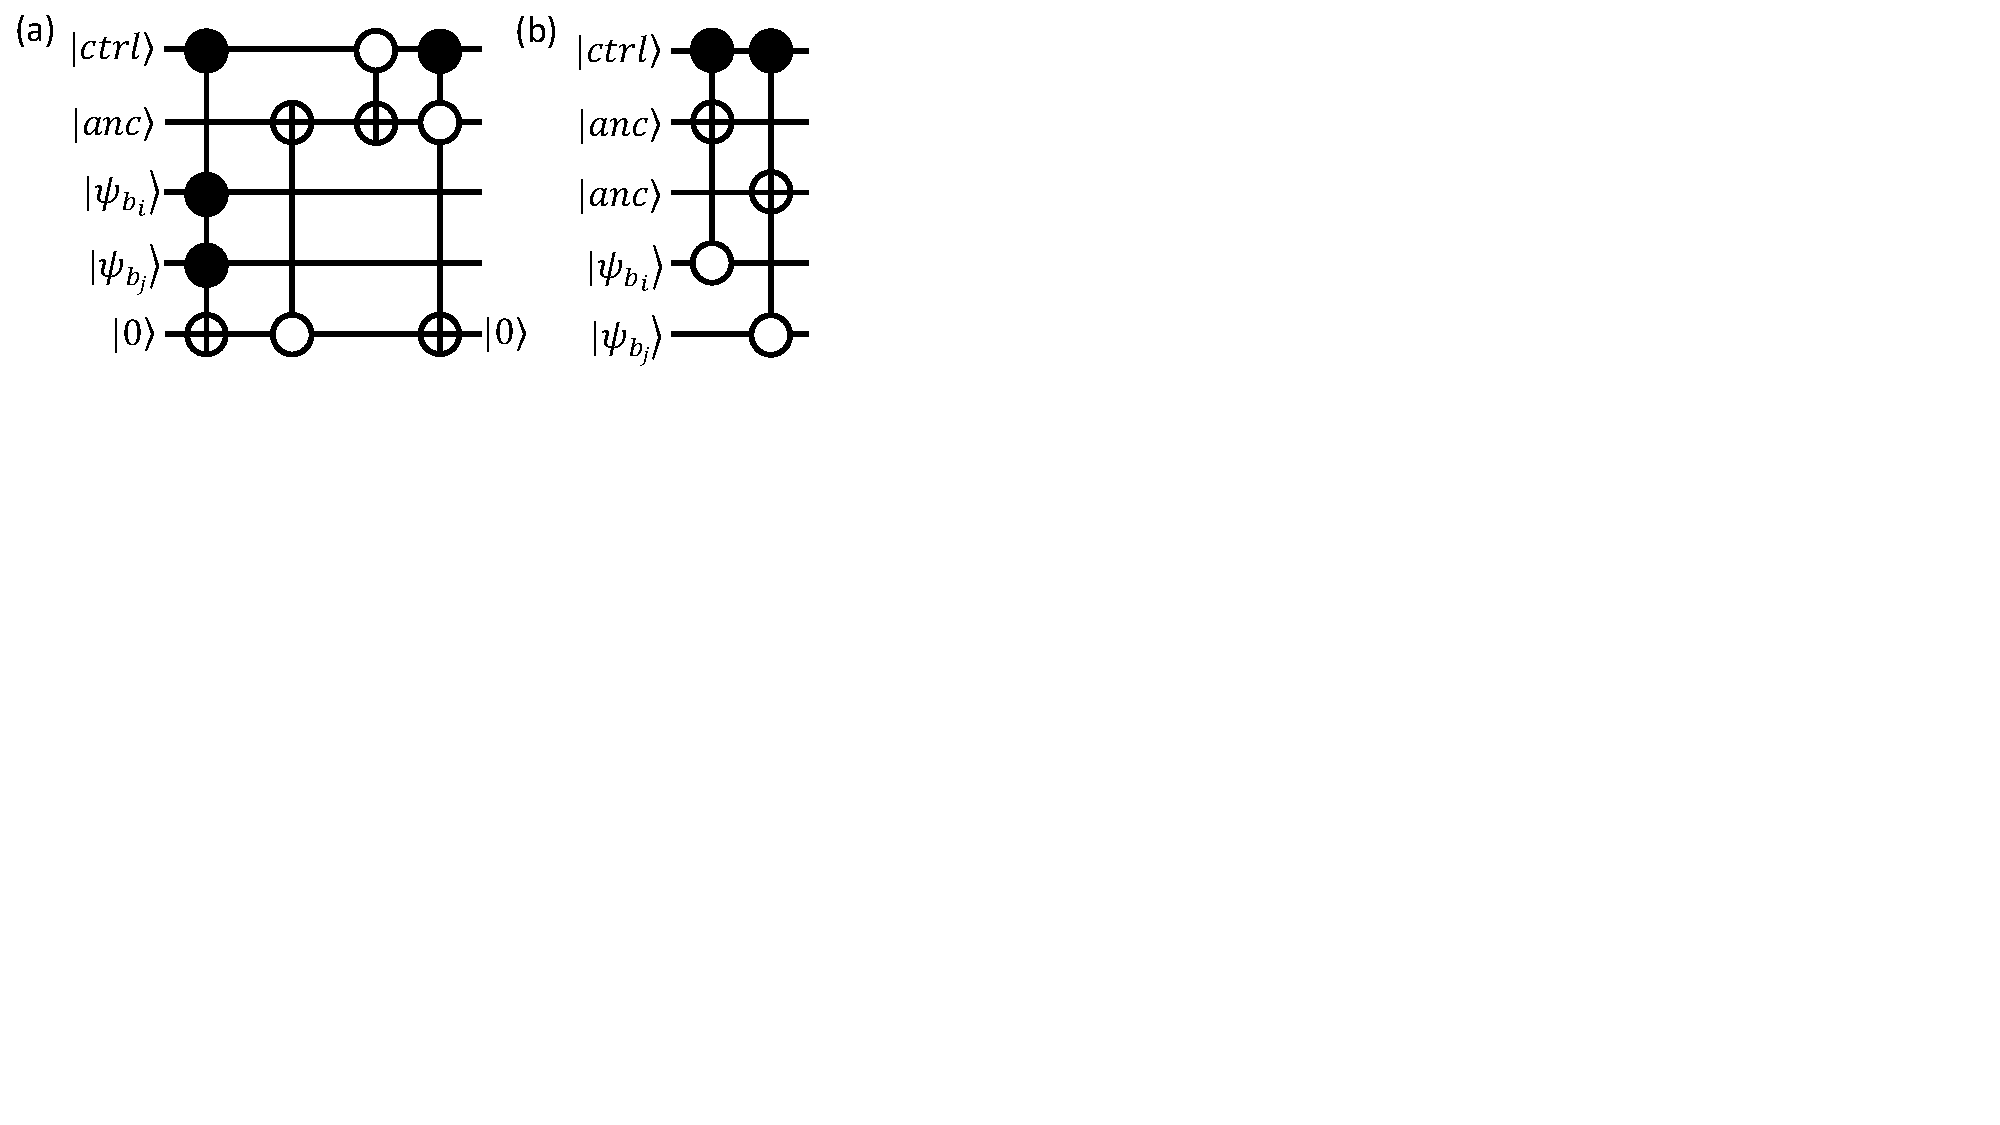
\includegraphics[width=8cm]{figures/fermionic-number-op-be.pdf}
    \caption{
        \textbf{Block-Encoding Products of Fermionic Number Operators}
        Two different constructions for block-encoding the operator $b_i^\dagger b_i b_j^\dagger b_j$ with $i \neq j$ are shown.
        The construction in subfigure a requires three Toffoli gates and one block-encoding ancilla while the construction in subfigure b requires two Toffoli gates and two block-encoding ancilla.
    }
    \label{fig:fermionic-number-op-be}
\end{figure}


In the case where each active fermionic mode has only a number operator acting on it we can construct block-encoding circuits in two different ways with a space-time tradeoff.
As an example, consider the product between two number operators: $b_i^\dagger b_i b_j^\dagger b_j$ with $i \neq j$.
Using the construction noted directly above, we can block-encode these operators using $B + 1$ Toffoli gates and one block-encoding ancilla.
This construction is shown in subfigure \ref{fig:fermionic-number-op-be}a.
Alternatively, we can use a product of the block-encoding circuits for the individual number operators shown in Figure \ref{fig:fermionic-be}a.
This construction requires $B$ Toffoli gates and $B$ block-encoding ancillae.
In the scenario where the number of block-encoding ancillae is not a limiting factor, then this construction may be preferred.
This construction is shown in subfigure \ref{fig:fermionic-number-op-be}b.

A natural question to ask is how do these constructions compare with using an LCU block-encoding after applying the Jordan-Wigner transformation \cite{}?
The Jordan-Wigner transformation maps each fermionic ladder operator (or number operator) to a sum of two Pauli operators.
For an arbitrary product of fermionic ladder operators, expanding these linear combinations results in $2^{B}$ Paulis.
The number of non-Clifford gates for LCU scales linearly with the number of operators and hence would scale exponentially with $B$ under this construction.

Alternatively, one could use LCU to construct individual block-encodings for each of the ladder operators in a term by applying the Jordan-Wigner transformation to each ladder operator (or number operator) independently.
The product of these block-encodings would then give a block-encoding of the term.
For each ladder operator (or number operator), an LCU block-encoding would require one Toffoli gate and one ancilla qubit.
In total, a block-encoding of the whole term using this construction would then require $B$ Toffoli gates and $B$ ancillae. 


\subsection{Linear Combinations of Fermionic Ladder Operators}

In the previous subsections, we presented block-encoding constructions for products of fermionic ladder operators.
In subsection \ref{subsec:lco}, we discussed a framework termed LCO which can be used to construct block-encodings for linear combinations of operators.
In this subsection, we will give quantum circuit constructions that block-encode specific linear combinations of products of fermionic ladder operators using fewer quantum resources than would be required using a naive LCO construction.

For a simple example, consider the case of a linear combination of an individual fermionic ladder operator with its hermitian conjugate: $b_i^\dagger + b_i$.
An LCO construction using the block-encodings for these two ladder operators individually would have a rescaling factor of $2$ and would require additional block-encoding ancillae and Toffoli gates to index between the two operators.
Alternatively, we can consider the action of the joined operator on the two possible occupation states of the $i^\text{th}$ fermionic mode:
\begin{equation}
    \begin{split}
        (b_i^\dagger + b_i) \ket{\psi_{b_i}} = \begin{cases} 
            \ket{1} & \text{when $\ket{\psi_{b_i}}$ is $\ket{0}$} \\
            \ket{0} & \text{when $\ket{\psi_{b_i}}$ is $\ket{1}$} \\
                                        \end{cases}
    \end{split}
\end{equation}
From this perspective, it is obvious that a block-encoding for this linear combination of operators can be achieved simply using a Pauli X gate.
The rescaling factor is then reduced to $1$ and no block-encoding ancillae are required.

One might notice that this is the same construction one would arrive at using the Jordan-Wigner transformation of the above operators.
Again, it is natural to ask if we can construct block-encodings of similar linear combinations of products of fermionic ladder operators that would be more efficient than using the Jordan-Wigner transformation and an LCU block-encoding.

Consider the operator: $b_i^\dagger b_j^\dagger b_k^\dagger b_l^\dagger +  b_i b_j b_k b_l$.
For a general operator of this form, the Jordan-Wigner transformation would result in $2^{B - 1}$ Pauli operators.
Alternatively, if we consider the action of these operators on the occupation states of these fermionic modes and ignore the sign of the output state for a moment, we can infer than only two states will not be zeroed-out:
\begin{equation}
    \begin{split}
        (b_i^\dagger b_j^\dagger b_k^\dagger b_l^\dagger +  b_i b_j b_k b_l) \ket{\psi_{b_i}}\ket{\psi_{b_j}}\ket{\psi_{b_k}}\ket{\psi_{b_l}} = \begin{cases} 
            \ket{1111} & \text{when $\ket{\psi_{b_i}}\ket{\psi_{b_j}}\ket{\psi_{b_k}}\ket{\psi_{b_l}}$ is $\ket{0000}$} \\
            \ket{0000} & \text{when $\ket{\psi_{b_i}}\ket{\psi_{b_j}}\ket{\psi_{b_k}}\ket{\psi_{b_l}}$ is $\ket{1111}$} \\
            0 & \text{otherwise} \\
                                        \end{cases}
    \end{split}
\end{equation}
From this perspective, we can see that we can determine the desired action of this operator on the state by computing the parity between successive pairs of the active fermionic modes.

Let $a = \ket{\psi_{b_i}} \oplus \ket{\psi_{b_j}}$, $b = \ket{\psi_{b_j}} \oplus \ket{\psi_{b_k}}$, and $c = \ket{\psi_{b_k}} \oplus \ket{\psi_{b_l}}$.
These variables can be computed using pairs of CNOT gates targeting a clean ancilla controlled on the corresponding fermionic mode.
Using this information, the state will be zeroed-out by the operator \textit{unless} $a = b = c = \ket{0}$.
Additionally, if these conditions are all true, the state of the system should be updated by successively applying $\vec{Z}X$ operators to each of the active modes.
The clean ancillae used to store the values of $a$, $b$, and $c$ can be uncomputed trivially since flipping each occupation state will not change the parity between pairs of modes.
A circuit diagram for this block-encoding is shown in subfigue \ref{fig:fermionic-hc-example}.


These circuits can also be generalized to include any linear combination of a product of fermionic ladder operators with its hermitian conjugate. 
An example circuit diagram for these generalized block-encoding circuits is shown in subfigue \ref{fig:fermionic-hc-generalized}.

For number operators that are present within the operator, these modes are not included in the parity computations nor are the occupation states of the modes updated.
Instead, the operation is controlled on the corresponding mode being in the $\ket{1}$ state.

For the other active modes, we focus on the term with the left-most ladder operator being an annihilation operator.
For each mode that has a creation operator being applied, the parity computations are computed using a CNOT gate that is $0$-controlled on the corresponding mode.
Additionally, classical preproccesing is used to determine if a $CZ$ gate that is $0$-controlled on the $i^\text{th}$ fermionic mode and $1$-controlled on the ancilla indicating that the term will not zero-out the state should be included.
If $B$ represents the number of active modes in the term and $C$ represents the number of those modes with a number operator acting on them, then this CZ gate is present if and only if $(B - C) \text{ choose } 2$ is odd.
A further description of the reasoning behind this construction is given in Appendix \ref{sec:hermitian-conjugate-construction}.

In general, these block-encoding circuit will all have a rescaling factor of $1$, use one block-encoding ancilla, and require $B$ Toffoli gates.

\subsection{Individual Bosonic Ladder Operators}

\ws{
\begin{enumerate}
    \item Chosen encoding
    \item Bosonic cutoffs
\end{enumerate}
}

\subsection{Action}

\ws{
    \begin{enumerate}
        \item Desired action
        \item Define rescaled operators
        \item Applying bosonic coefficients 
        \item Updating Occupancy
        \item Applying single bosonic op
        \item Applying multiple bosonic operators on same mode
        \item Applying multiple bosonic operators on different modes
    \end{enumerate}
}

\subsection{Products of Bosonic Ladder Operators}


\subsection{Linear Combinations of Bosonic Ladder Operators}


\subsection{Products of Ladder Operators}

\ws{
    How do we apply a term?
    \begin{enumerate}
        \item Define rescaled term and applying rescaled term with updated coefficient
        \item Applying term by sequentially applying ladder-op oracles 
    \end{enumerate}
}